\subsubsection{Tour improvement}

Improvement heuristics are algorithms which work over a valid and complete solution
in order to improve it.
The most commom improvement heuristics are the 2-opt and 3-opt
local search algorithms.
The Lin-Kernighan algorithm (LKA) is a particular implementation of the
above mentioned local searches methods, in which a $k$-opt local search is employed,
where the value of $k$ varies during the algorithm execution.
LKA have shown to be very efficient and capable of presenting high quality solutions to the TSP.


%----------------------------
\paragraph{2 and 3 opt tours}
"In optimization, 2-opt is a simple local search algorithm first proposed
by Croes in 1958 for solving the traveling salesman problem."

The 2-opt is possibly the most simple local search algorithm. The objective
of this method is to find route crossovers, and fold them. When this occurs,
the overal cost of the newly constructed tour will decrease.

The 2-opt search works in a recursive way.
This search algorithm tries to improve the original tour, by removing two
edges from the original cycle, and reconnecting the two paths created.
This process is ilustrated in figure $\ref{fig:two_opt_move}$.
In a 2-opt search, there is only one way of connecting the nodes in a way
which will result in a different and valid tour.
If the new tour has a lower cost, the cycle restarts, using the new tour
as the improvement object.
Otherwise, two other edges are selected, and the cycle continues with
the original solution.
This iterative method continues untill no further improvement is reached
over a complete iteration cycle. In this case, the tour is known to be 2-opt.

\begin{figure}[htpb]
  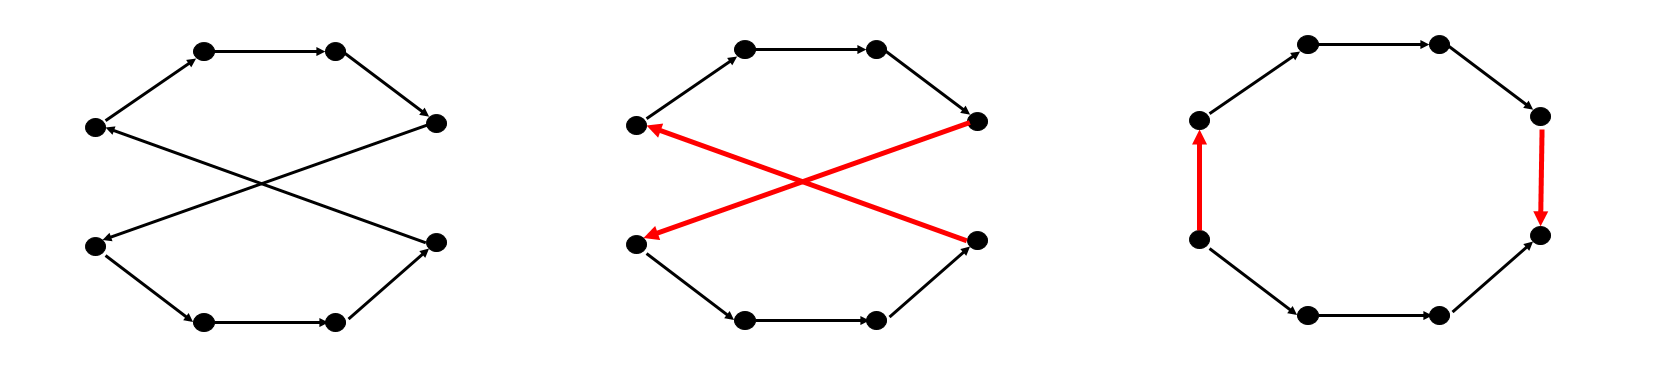
\includegraphics[scale=0.3]{./Figures/tsp/2-opt-explained}
  \caption{The 2-opt local search works by reconnecting two edges, hoping to
  fold possible crossovers, decreasing the overall tour coust. In the left image,
  a crossover is identified. In the middle image, a the edges beloning to this crossover
  are removed, and in the figure to the right, they are reconnected, forming a new valid tour}
  \label{fig:two_opt_move}
\end{figure}

The 3-opt search is very similar to the 2-opt. Instead of selecting
two edges and reconnecting the path, the 3-opt selects 3 edges. In this case,
there are two different ways of forming a new valid tour. A 3-opt move
can also be seen as two or three 2-opt moves combined in the formation of a
new tour. The iterative cycle of the 3-opt search works in the same way as
the 2-opt.






%----------------------------
\paragraph{k opt tour}
More generally, $k$-opt local search methods are a way of rearanging a tour,
by taking $k$ edges and reconnecting the paths in order to form a new valid tour.
Any tour that is known to be $k-opt$ is also $(k-1)opt$. Some particular problems,
as "the crossing bridges", figure $\ref{fig:crossing_bridges}$ can only be solved with a 4-opt or higher method.

\begin{figure}[htbp]
  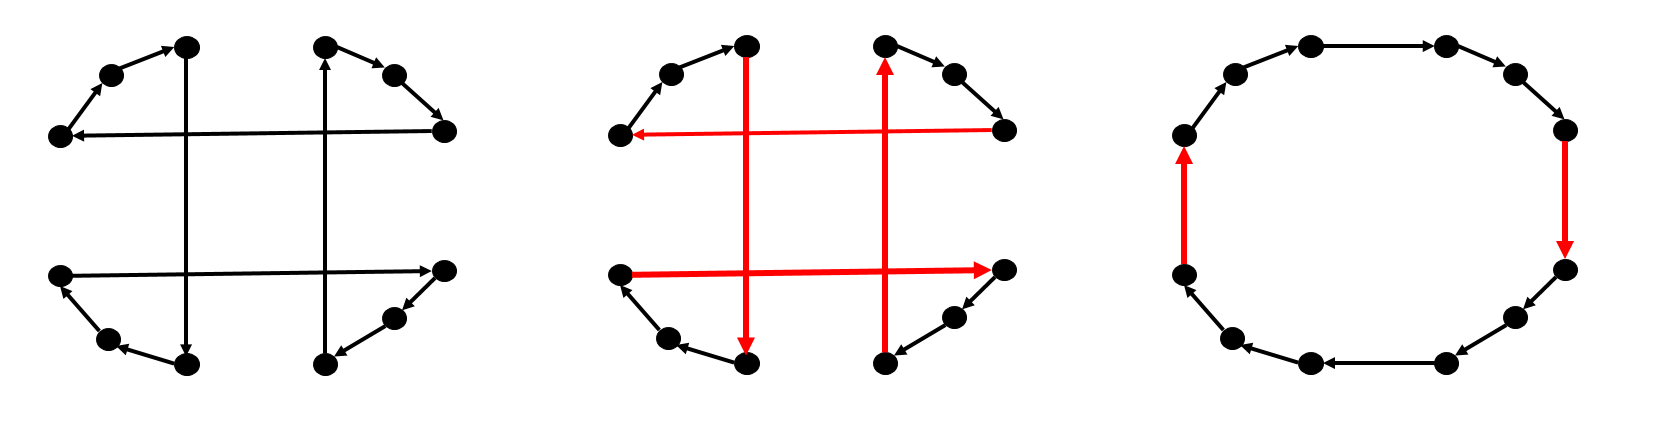
\includegraphics[scale=0.3]{./Figures/tsp/crossing_bridges}
  \caption{The crossing bridges can only be solved by reordering 4 edges.
  The resolution of this problem with local search is only possible
  with 4-opt or higher.}
  \label{fig:crossing_bridges}
\end{figure}


\paragraph{Lin-Kernighan heuristic}

The Lin-Kernighan Heuristic (LKH) \cite{lkh_original}, is an algorithm for the symmetric TSP, 
which was the state of the art for over than 15 years.
LKH is known for producing optimal solutions often, for presenting solutions within 2$\%$ of the Held-Karp lower bound, 
and for having a time complexity of approximately $\mathcal{O}^{n^{2.2}}$, \cite{heuristics_tsp}.
This heuristic is constructed for the symmetric, and using it for the asymmetric generalization requires a 
graph tranformation process, which transforms the asymmetric instance with $n$ nodes, into an equivalent symmetric one with $2n-1$ nodes, \cite{atsp_to_tsp_1} \cite{atsp_to_tsp_2}.
Thus, for the same number of nodes, solving an assymetric TSP with the LKH heuristic is usually 4 times harder than solving the symmetric case.

To understand the Lin-Kernighan heuristic, it is necessary to think about the TSP in a slighly different manner.
Consider the following way of defining a combinatorial optimization problem: "find from a set
$S$ a subset $T$ that satisfies some criterion $C$ and minimizes an objective function $f$."
In the TSP, the objective is to find from the set of all edges ($S$) of a complete graph,
the subset ($T$) which forms a valid tour ($C$) and minimizes the objective function ($f$). 
Using this formulation it is now possible to explain the LK heuristics.

Given an non-optimal and feasible solution $T$, it is non-optimal because $k$ elements $\{x_1, ..., x_k\}$ in T are \textit{out of place}.
To improve this solution, and make it optimal, one would have to substitue the set of $k$ elements $x_1, ..., x_k$
with the elements $y_1, ..., y_k$ of $S \backslash T$. Because there is no knowledge about how many elements are missplaced,
Lin and Kernighan consider that setting the value of $k$ a-priori would seem artificial. 
Thus, they propose an interative procedure in which the algorithm dynamically estimates the best value for $k$.
In order to do this, the LKH first estimates the most out of place elements, $x_1$ and $y_1$. Then,
with this values set aside, it tries to repeat this proccess for $x_2$ and $y_2$, and so on. It stops this inner loop 
when no improvement seams plausible, replaces the current solution $T$ with the new solution generated from replacing the now selected elements,
and restarts the whole proccess. This proccess is formalized below, as presented by Lin and Kernighan.

This heuristic has not been shown to work for the time-dependent TSP, as it is constructed for a symmetrical $n*n$ cost matrix only.
Thus, the overview of this algorithm will not be extensive, as it has no pratical application to the problem under consideration.
In any case, being a very relevant heuristic for the classical TSP, it is an algorithm worth mentioning.


